% This paper uses LLNCS macro package for Springer Computer Science proceedings;
% Version 2.20 of 2017/10/04
%
\documentclass[runningheads]{llncs}
%
\usepackage{subcaption}
\captionsetup{compatibility=false}
\usepackage{graphicx}
\usepackage{placeins}
\usepackage{float}
% Used for displaying a sample figure. If possible, figure files should
% be included in EPS format.
%
% If you use the hyperref package, please uncomment the following line
% to display URLs in blue roman font according to Springer's eBook style:
% \renewcommand\UrlFont{\color{blue}\rmfamily}

\begin{document}
%
\title{Immortals 2024 Extended Team Description Paper}
\titlerunning{Immortals 2024 ETDP}

\author{Ali Salehi \and
Mohammad Tabasi \and
Omid Najafi \and
Ali Amoozandeh Nobaveh \and
MohammadHossein Fazeli \and
MohammadAli Ghasemieh \and
MohammadReza Niknezhad \and
Mustafa Talaeezadeh}
%
\authorrunning{Immortals Robotics}
%
\institute{
\url{http://www.immortals-robotics.com}
}
%
\maketitle              % typeset the header of the contribution
%
\begin{abstract}
This paper describes the recent work that has been done by the Immortals Robotics Team for the upcoming RoboCup 2024 competition in Eindhoven, Netherland.

\keywords{RoboCup 2024 \and Small Size League}
\end{abstract}

\section{Introduction}
The Immortals Small Size League team was founded in 2008. We first participated in RoboCup 2009 in Graz. Later, we won several awards. This included 2nd place in RoboCup 2011 in Istanbul, and 3rd place in RoboCup 2023 in Bordeaux. The team currently consists of computer and electrical engineers.

In the past year, our team focused on updating the electronics and software structure \cite{ref_ETDP2023}. These changes were aimed at improving the core functionalities of our system. While these updates represented a major step forward, they also introduced significant instability. Consequently, we were compelled to revert some parts of the system to older designs during RoboCup 2023.

This year, our main focus will shift to enhancing system robustness. We will also capitalize on the improved hardware and software foundation established through modernization efforts. By prioritizing robustness enhancement, we aim to ensure a more stable and reliable performance of our system in future competitions.
 
It is worth mentioning that we will publish our designs and software on our GitHub page \cite{ref_github} shortly after the competition is over.

\begin{figure}
    \centering
    \begin{subfigure}[b]{0.45\textwidth}
         \centering
         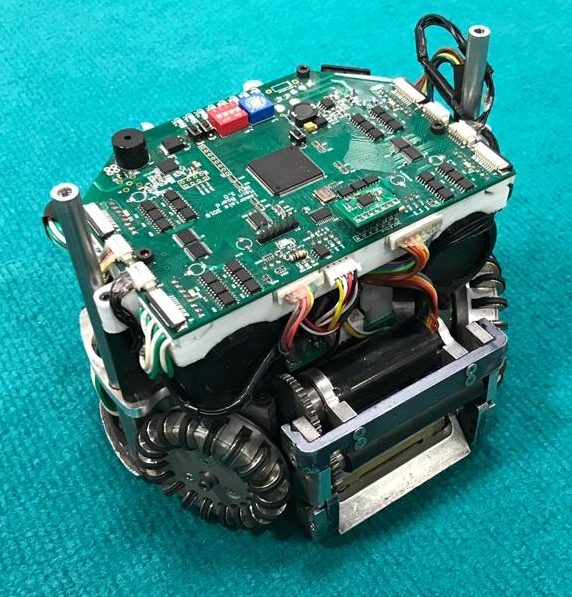
\includegraphics[width=\textwidth]{images/std_robot.jpeg}
         \caption{Standard}
         \label{fig:robot_std}
    \end{subfigure}
    \hfill
    \begin{subfigure}[b]{0.5\textwidth}
        \centering
        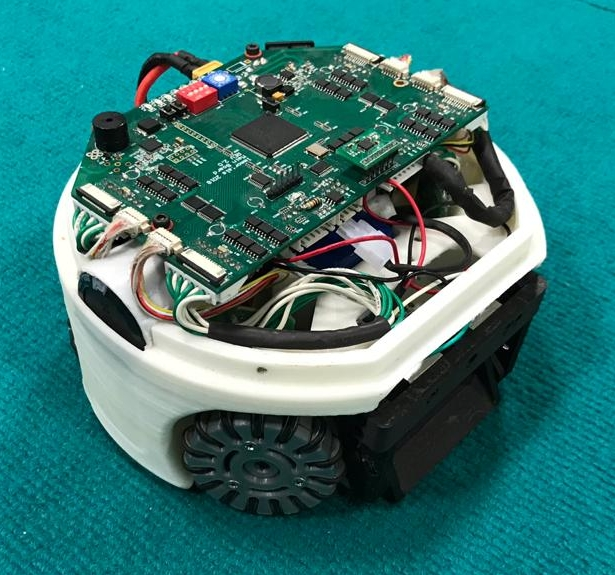
\includegraphics[width=\textwidth]{images/printed_robot.jpeg}
        \caption{3D-printed}
        \label{fig:robot_printed}
    \end{subfigure}
    \caption{Immortals current robots.}
    \label{fig:robots}
\end{figure}

\section {Mechanics}
The mechanical design team decided not to overhaul the entire system. Instead, they chose to modify design details due to the optimal design of the previous robots. This change aims to improve the manufacturability and durability of the parts. Recent advances in additive manufacturing techniques have made 3D-printed parts more accurate and reliable. This is driving our developments toward broader use of these elements. We're also replacing several mechanical parts made using traditional methods, such as turning and wire EDM, with additively manufactured parts. This will cut costs and speed up manufacturing and maintenance.

Manufacturing companies are consulted on the technical drawings of the revised design. Most of the manufacturing work for the new series of robots has been outsourced.

\section{Electronics}

\indent Last year, we redesigned all of our electronics from scratch to reflect the latest developments in the league and also in the industry. The main goals were:

\begin{enumerate}
    \item[$\bullet$] reliability
    \item[$\bullet$] expandability
    \item[$\bullet$] being more competitive
\end{enumerate}

After writing last year's TDP and during the design and prototyping phase, we made several changes to the architecture that can be seen in Fig. \ref{fig:electronics-architecture}. These changes will be described in the following sections.

\begin{figure}
	\centering
	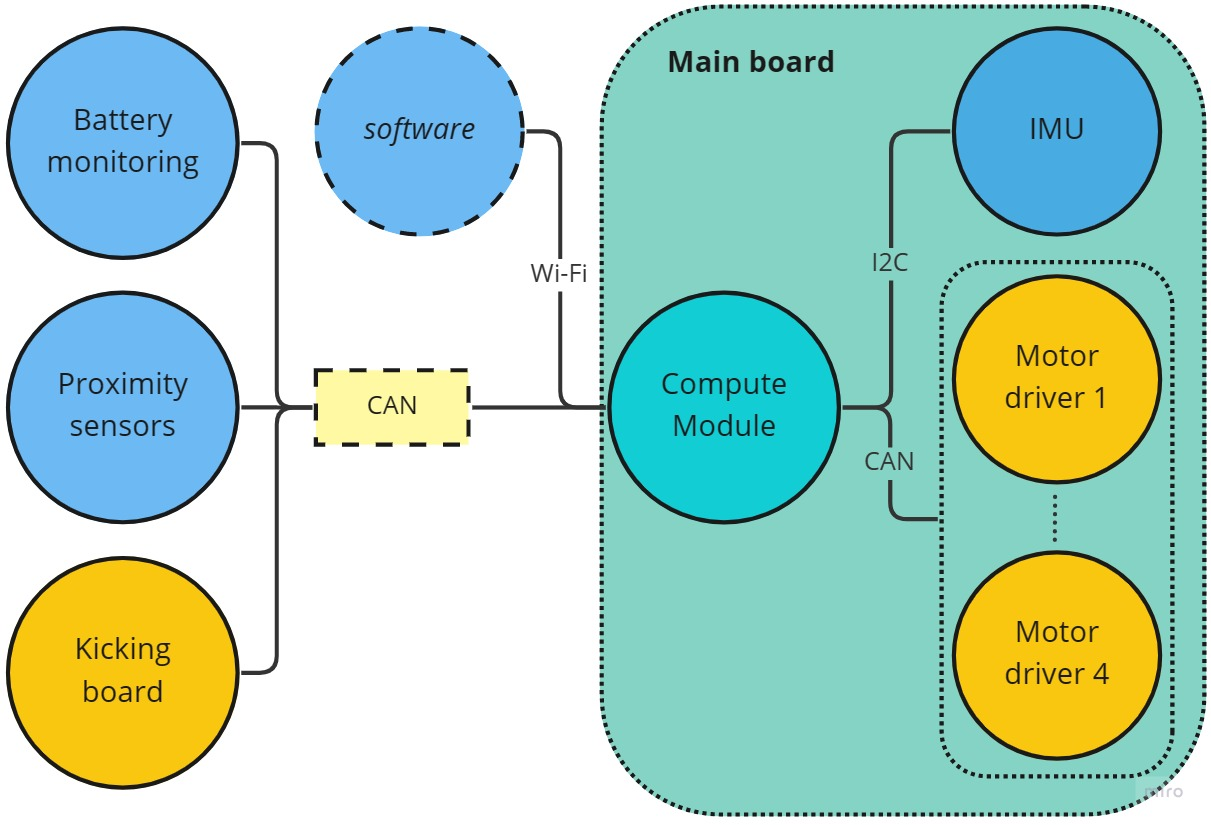
\includegraphics[width=0.8\textwidth]{images/electronics-architecture.jpg}
	\caption{Revised electronics architecture}
	\label{fig:electronics-architecture}
\end{figure}

it's important to highlight that the new designs worked well and addressed many of the issues we faced before. However, the changes also added far more complexity to the system. Additionally, the global chip shortage, especially for the Compute Module, made it hard to get all the components we needed. As a result, we weren't able to use the new boards for half of our robots like we had planned.

\subsection{Main board}

Our current main board (Fig. \ref{fig:main-board}) was designed last year and uses a Raspberry Pi Compute Module (CM) 4 as the local compute unit on the robot. 

\begin{figure}
	\centering
	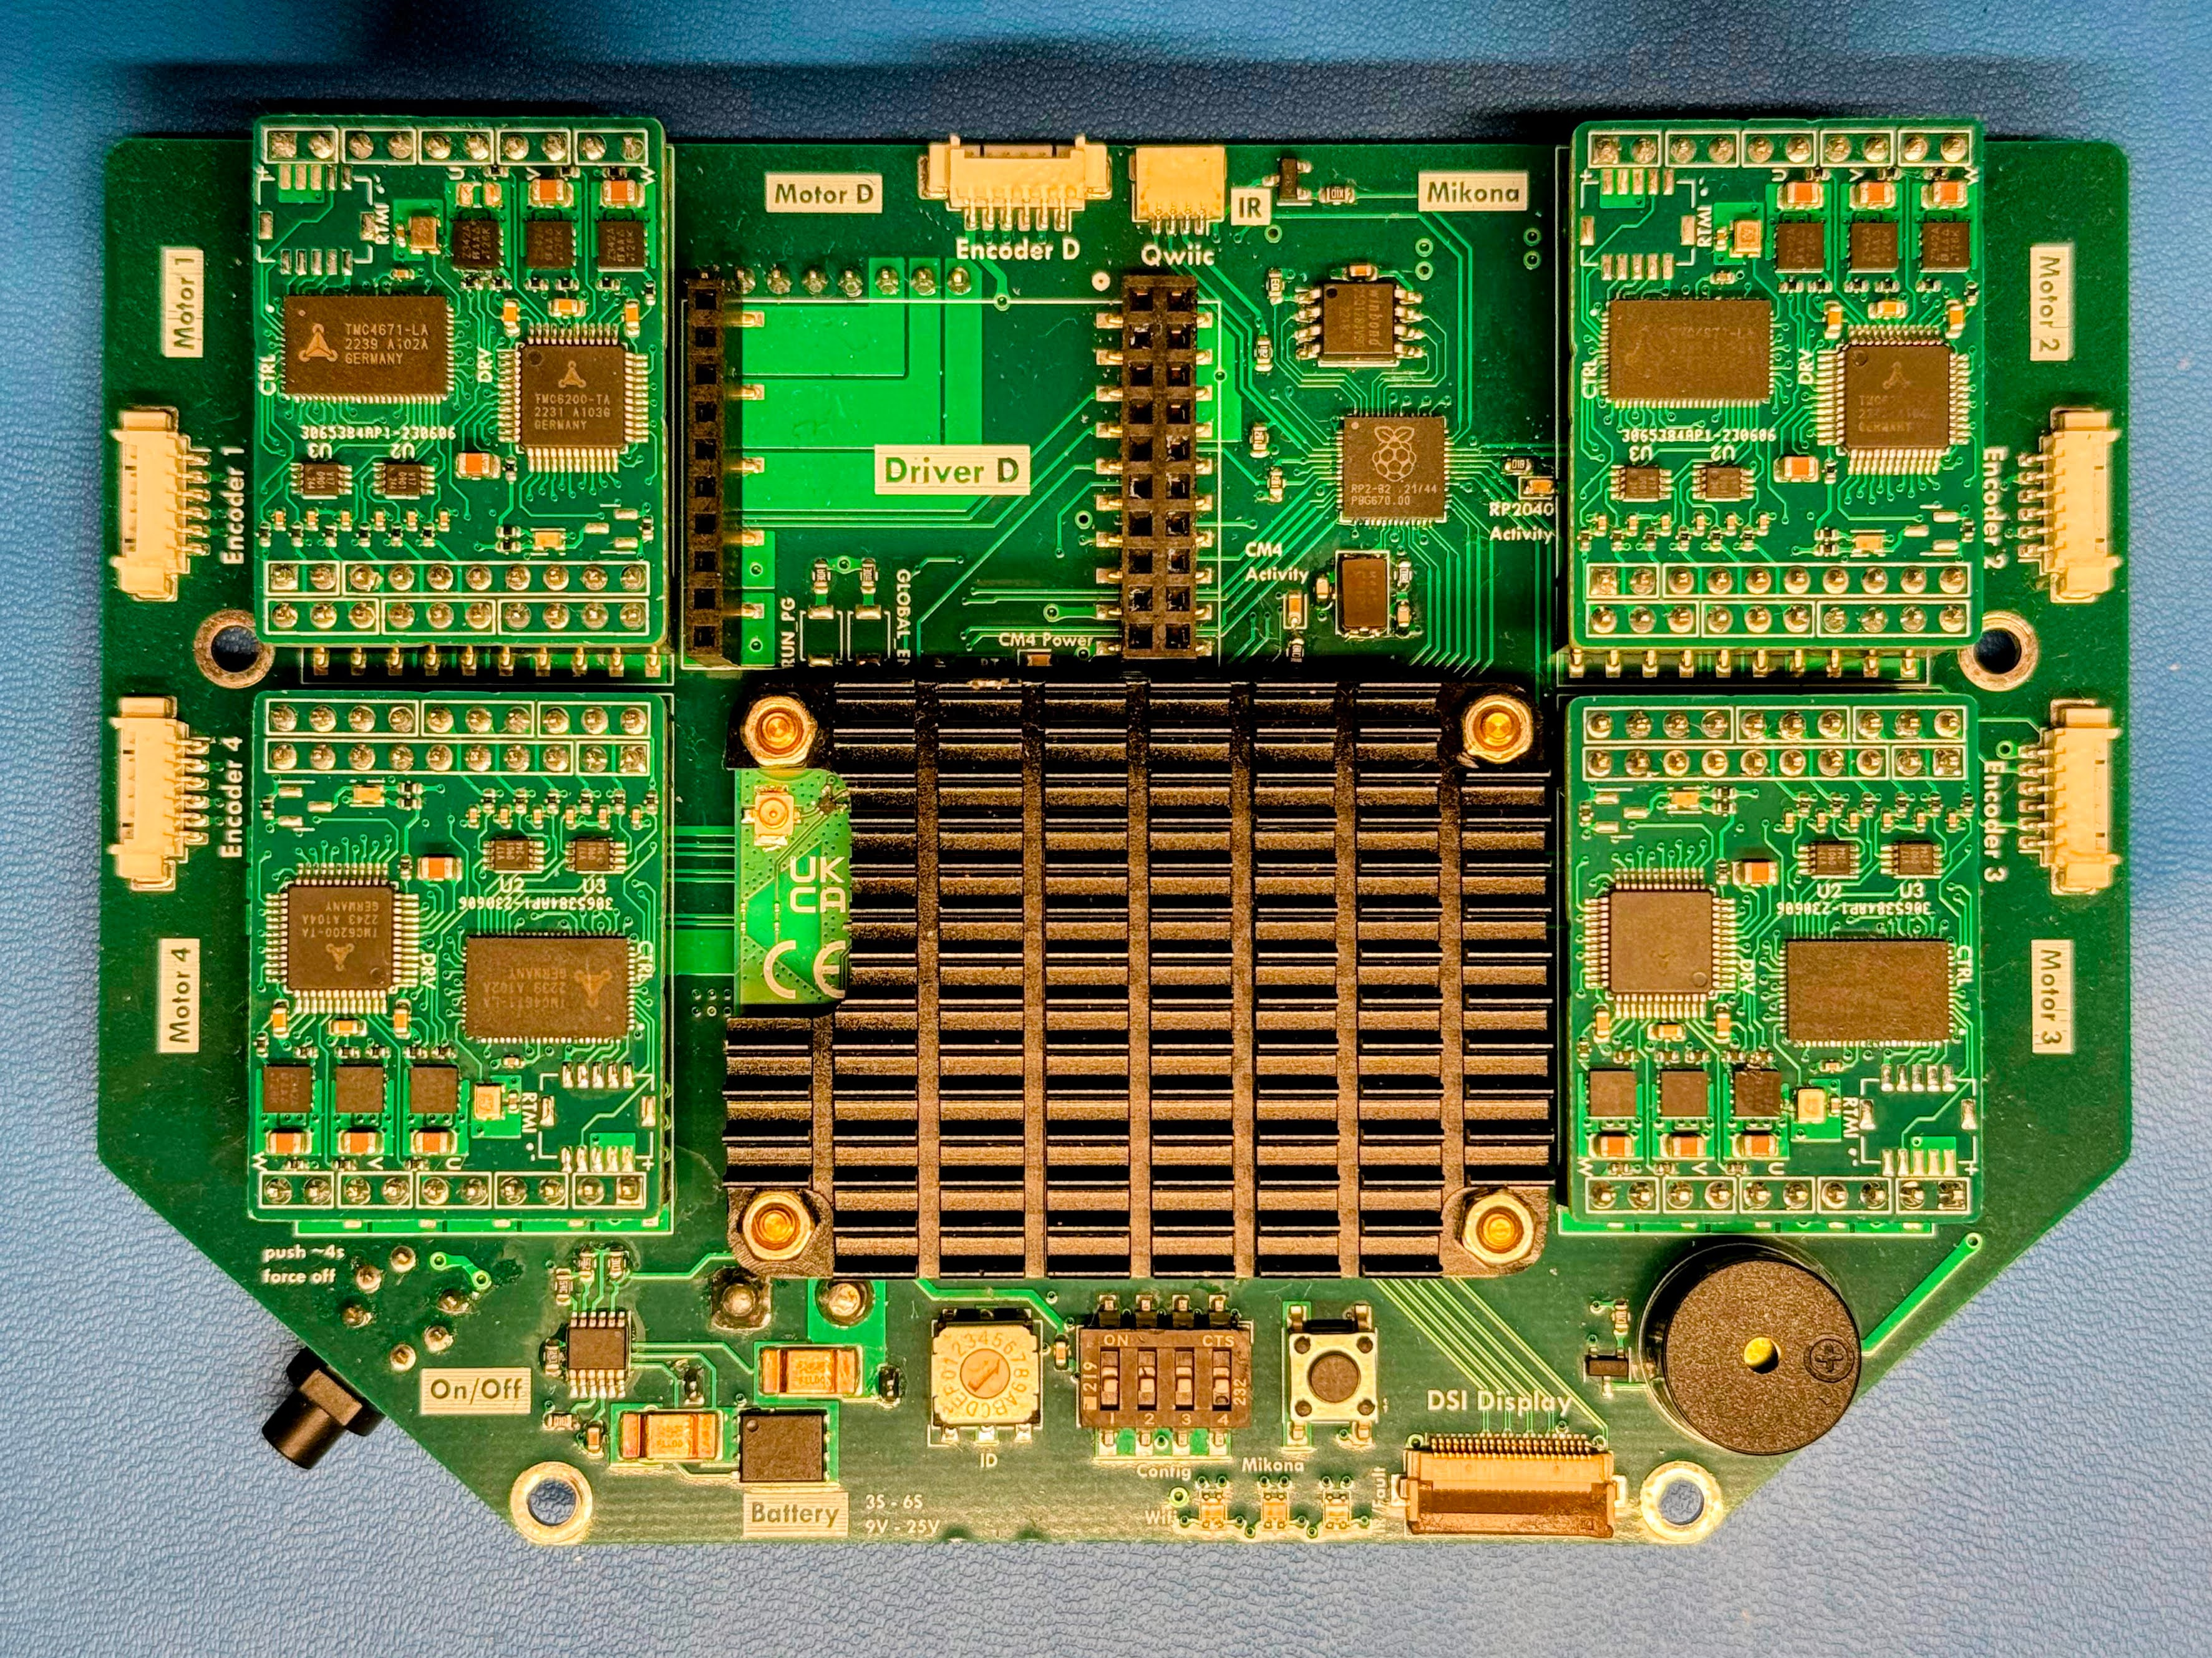
\includegraphics[width=0.8\textwidth]{images/main-board.jpg}
	\caption{New main board}
	\label{fig:main-board}
\end{figure}

We also use its 5GHz WiFi as the wireless communication link. During last year's competition we observed satisfactory results using it, with results very similar to what we had measured in the lab. Therefore we didn't follow with adding an additional nRf wireless link.

We made a design change after writing last year's TDP. Instead of using CAN, we now use Serial Peripheral Interface (SPI) to communicate with the motor controllers. The main reasons were simplicity and price. During development and testing, we couldn't find any issues with the simpler SPI bus that we hoped CAN could fix. The chip shortage caused the price of anything that speaks CAN to be much higher than in the past. The auto industry had priority over others for CAN-capable devices.

However, during the firmware implementation phase, we encountered significant challenges. We attempted to utilize the SPI bus on the Raspberry Pi for communication with the motor controllers. However, the speed of this interface fell considerably short of our expectations. We were using linux's builtin SPI driver, with Trionamic's API on top of it. This meant each byte were sent separately to the kernel causing a kernel mode switch every time. TODO: add some numbers and fact-check these.

This year we are using a manual implementation of the SPI bus, hoping that it would improve the performance.

\subsection{Motor driver}
Our motor drivers (Fig. \ref{fig:motor-driver}) are separate modules that sit on top of the main board. This greatly improves our ability to repair robots if one of the drivers fails. It also makes it easier to develop the main board and the motor drivers further separately.

\begin{figure}
	\centering
	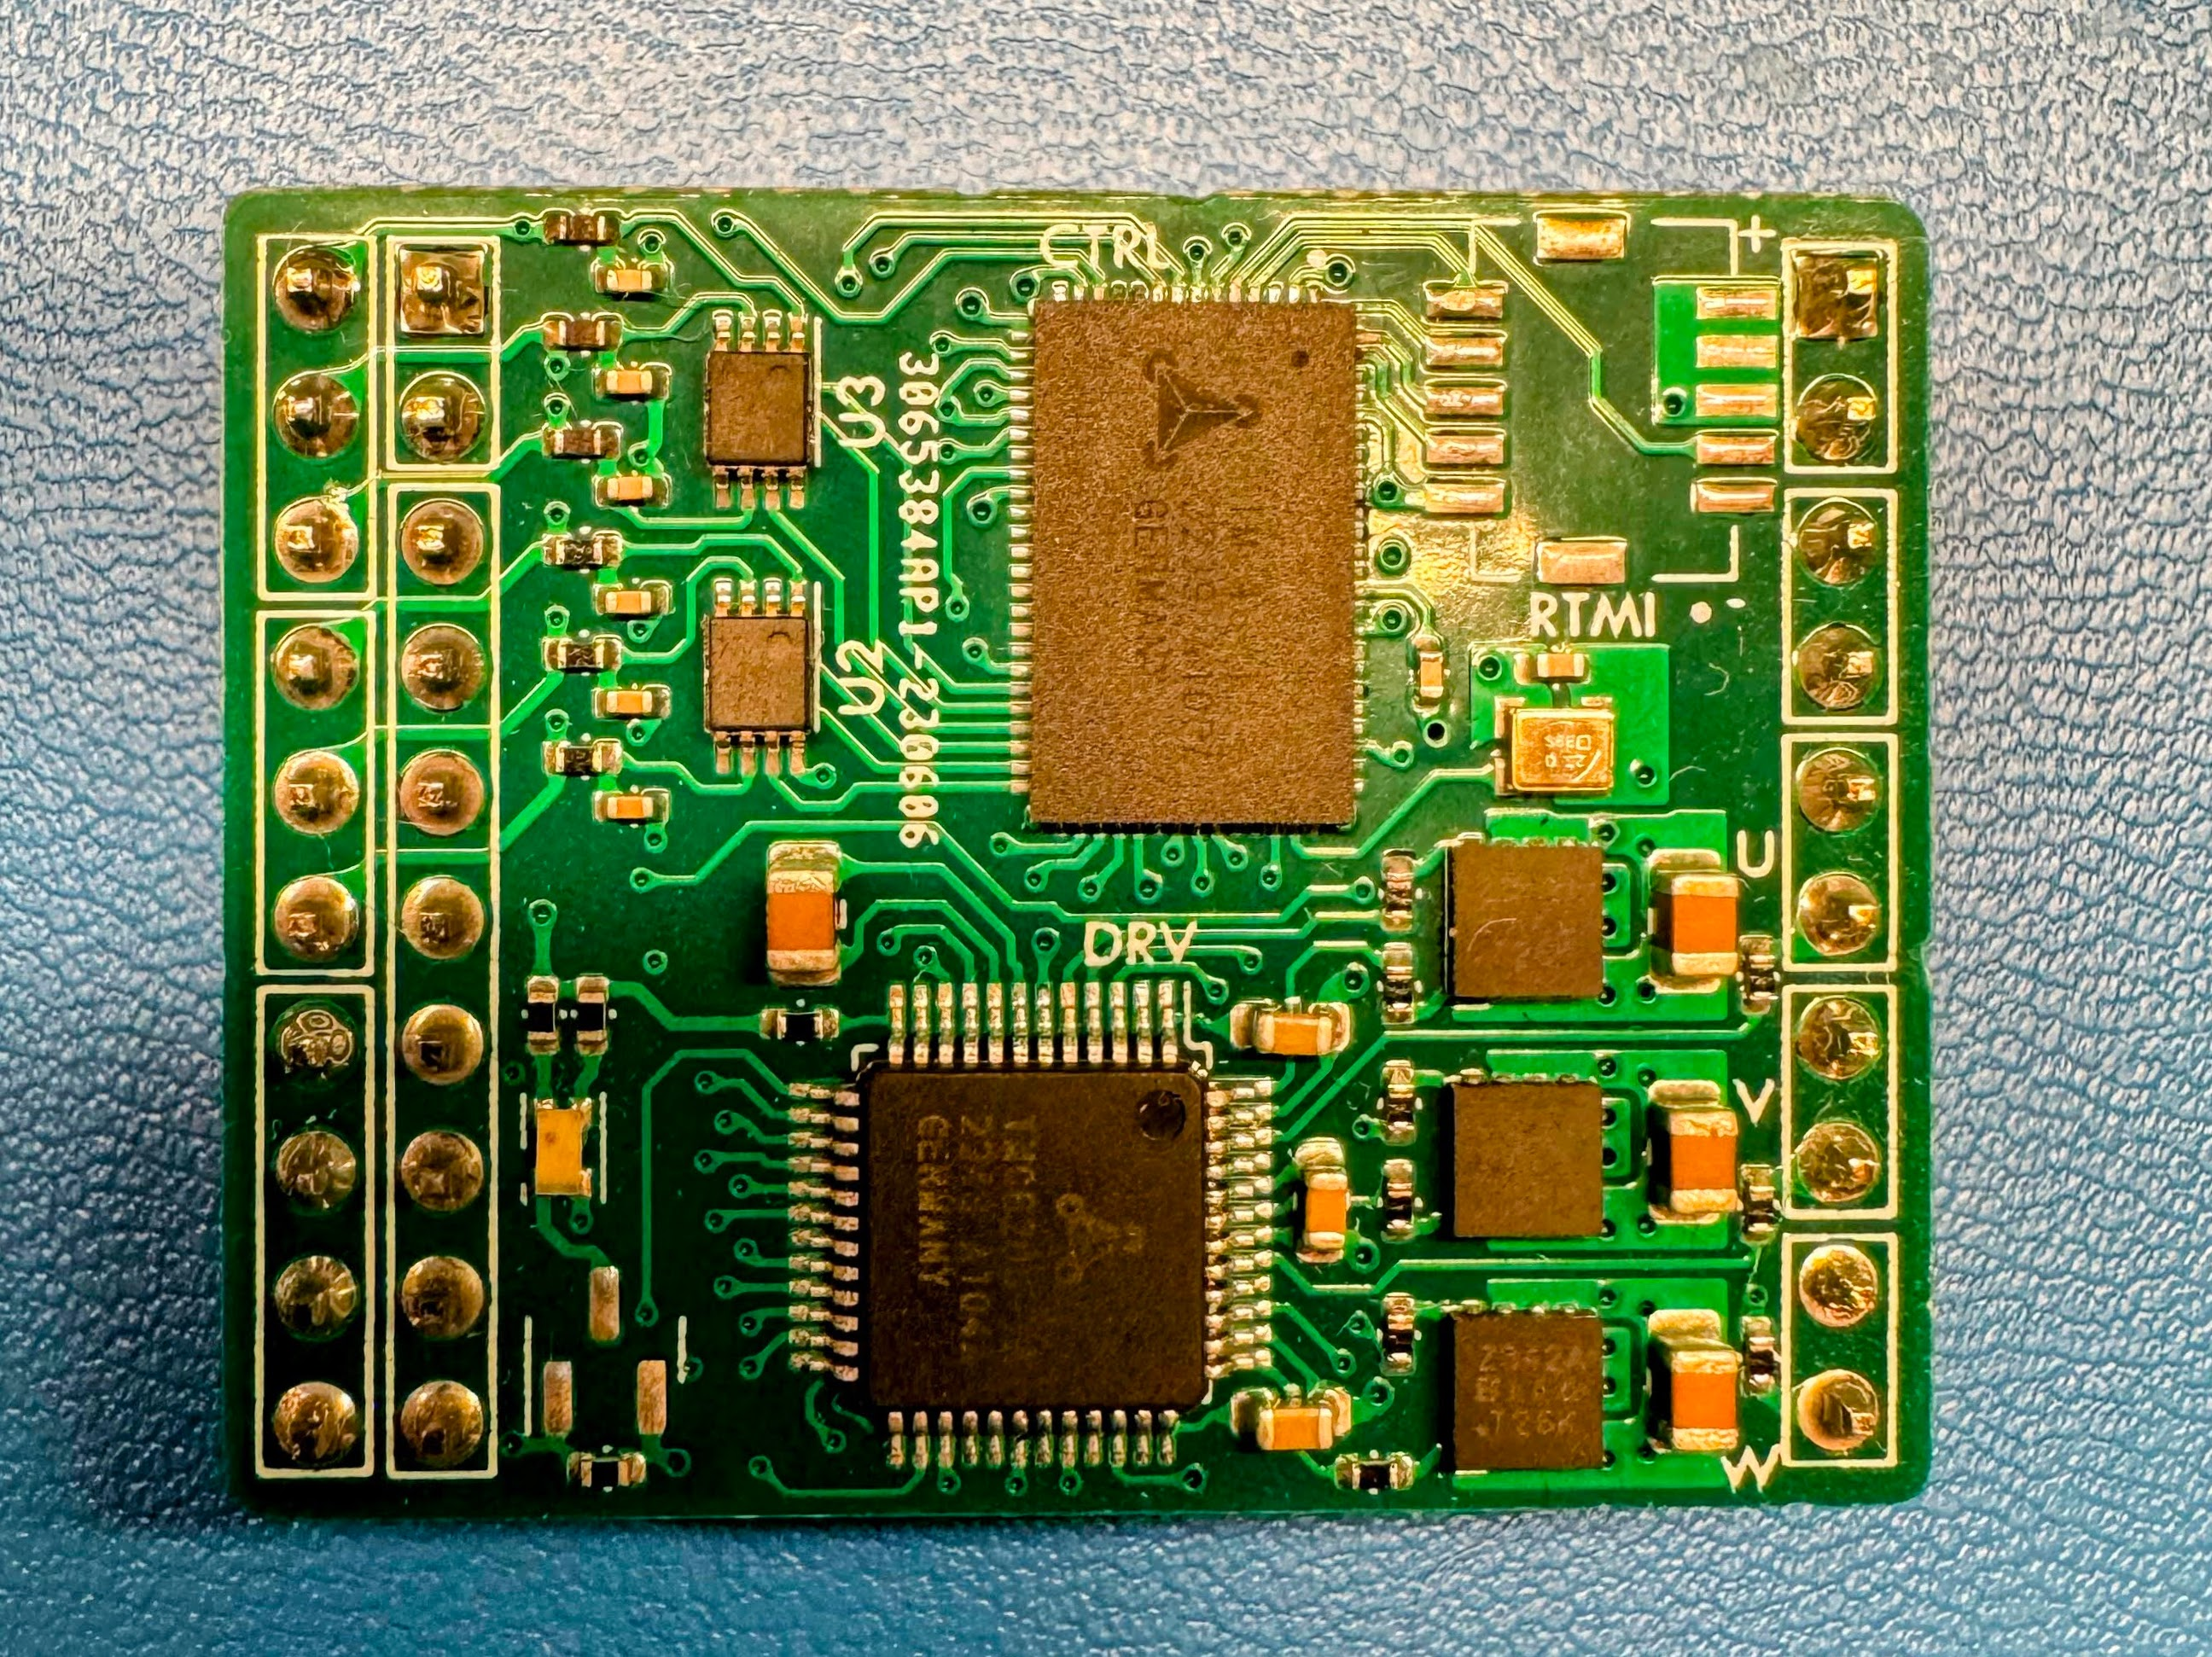
\includegraphics[width=0.8\textwidth]{images/motor-driver.jpg}
	\caption{The new motor driver module}
	\label{fig:motor-driver}
\end{figure}

We use a dedicated BLDC motor driver IC, TMC4671. It implements Field Oriented Control (FOC) for BLDC motors and includes various control methods. This offloads the local motor control functionality from the main processor to dedicated hardware, which is more reliable in terms of latency.

These drivers talk directly to the Compute Module using the SPI bus. They receive both configuration and commands, and send back sensor data including speed and position. We use the TMC-API (TODO: ref) from Trinamic to make it easier to read from and write to the TMC4671's registers.

We also use a power MOSFET driver IC, TMC6200. It drives the MOSFETs and senses the motor currents needed for the FOC algorithm. It also includes a fault detection mechanism. It shares the same SPI bus with TMC4671 and is directly connected to the Compute Module.

\subsection{Kicking board}
Our kicking board (Fig. \ref{fig:mikona}) uses a dedicated LT3570 flyback capacitor charger IC. It drives a BSC109N10NS3G MOSFET connected to a DA2034 transformer for this circuit.

\begin{figure}
    \centering
    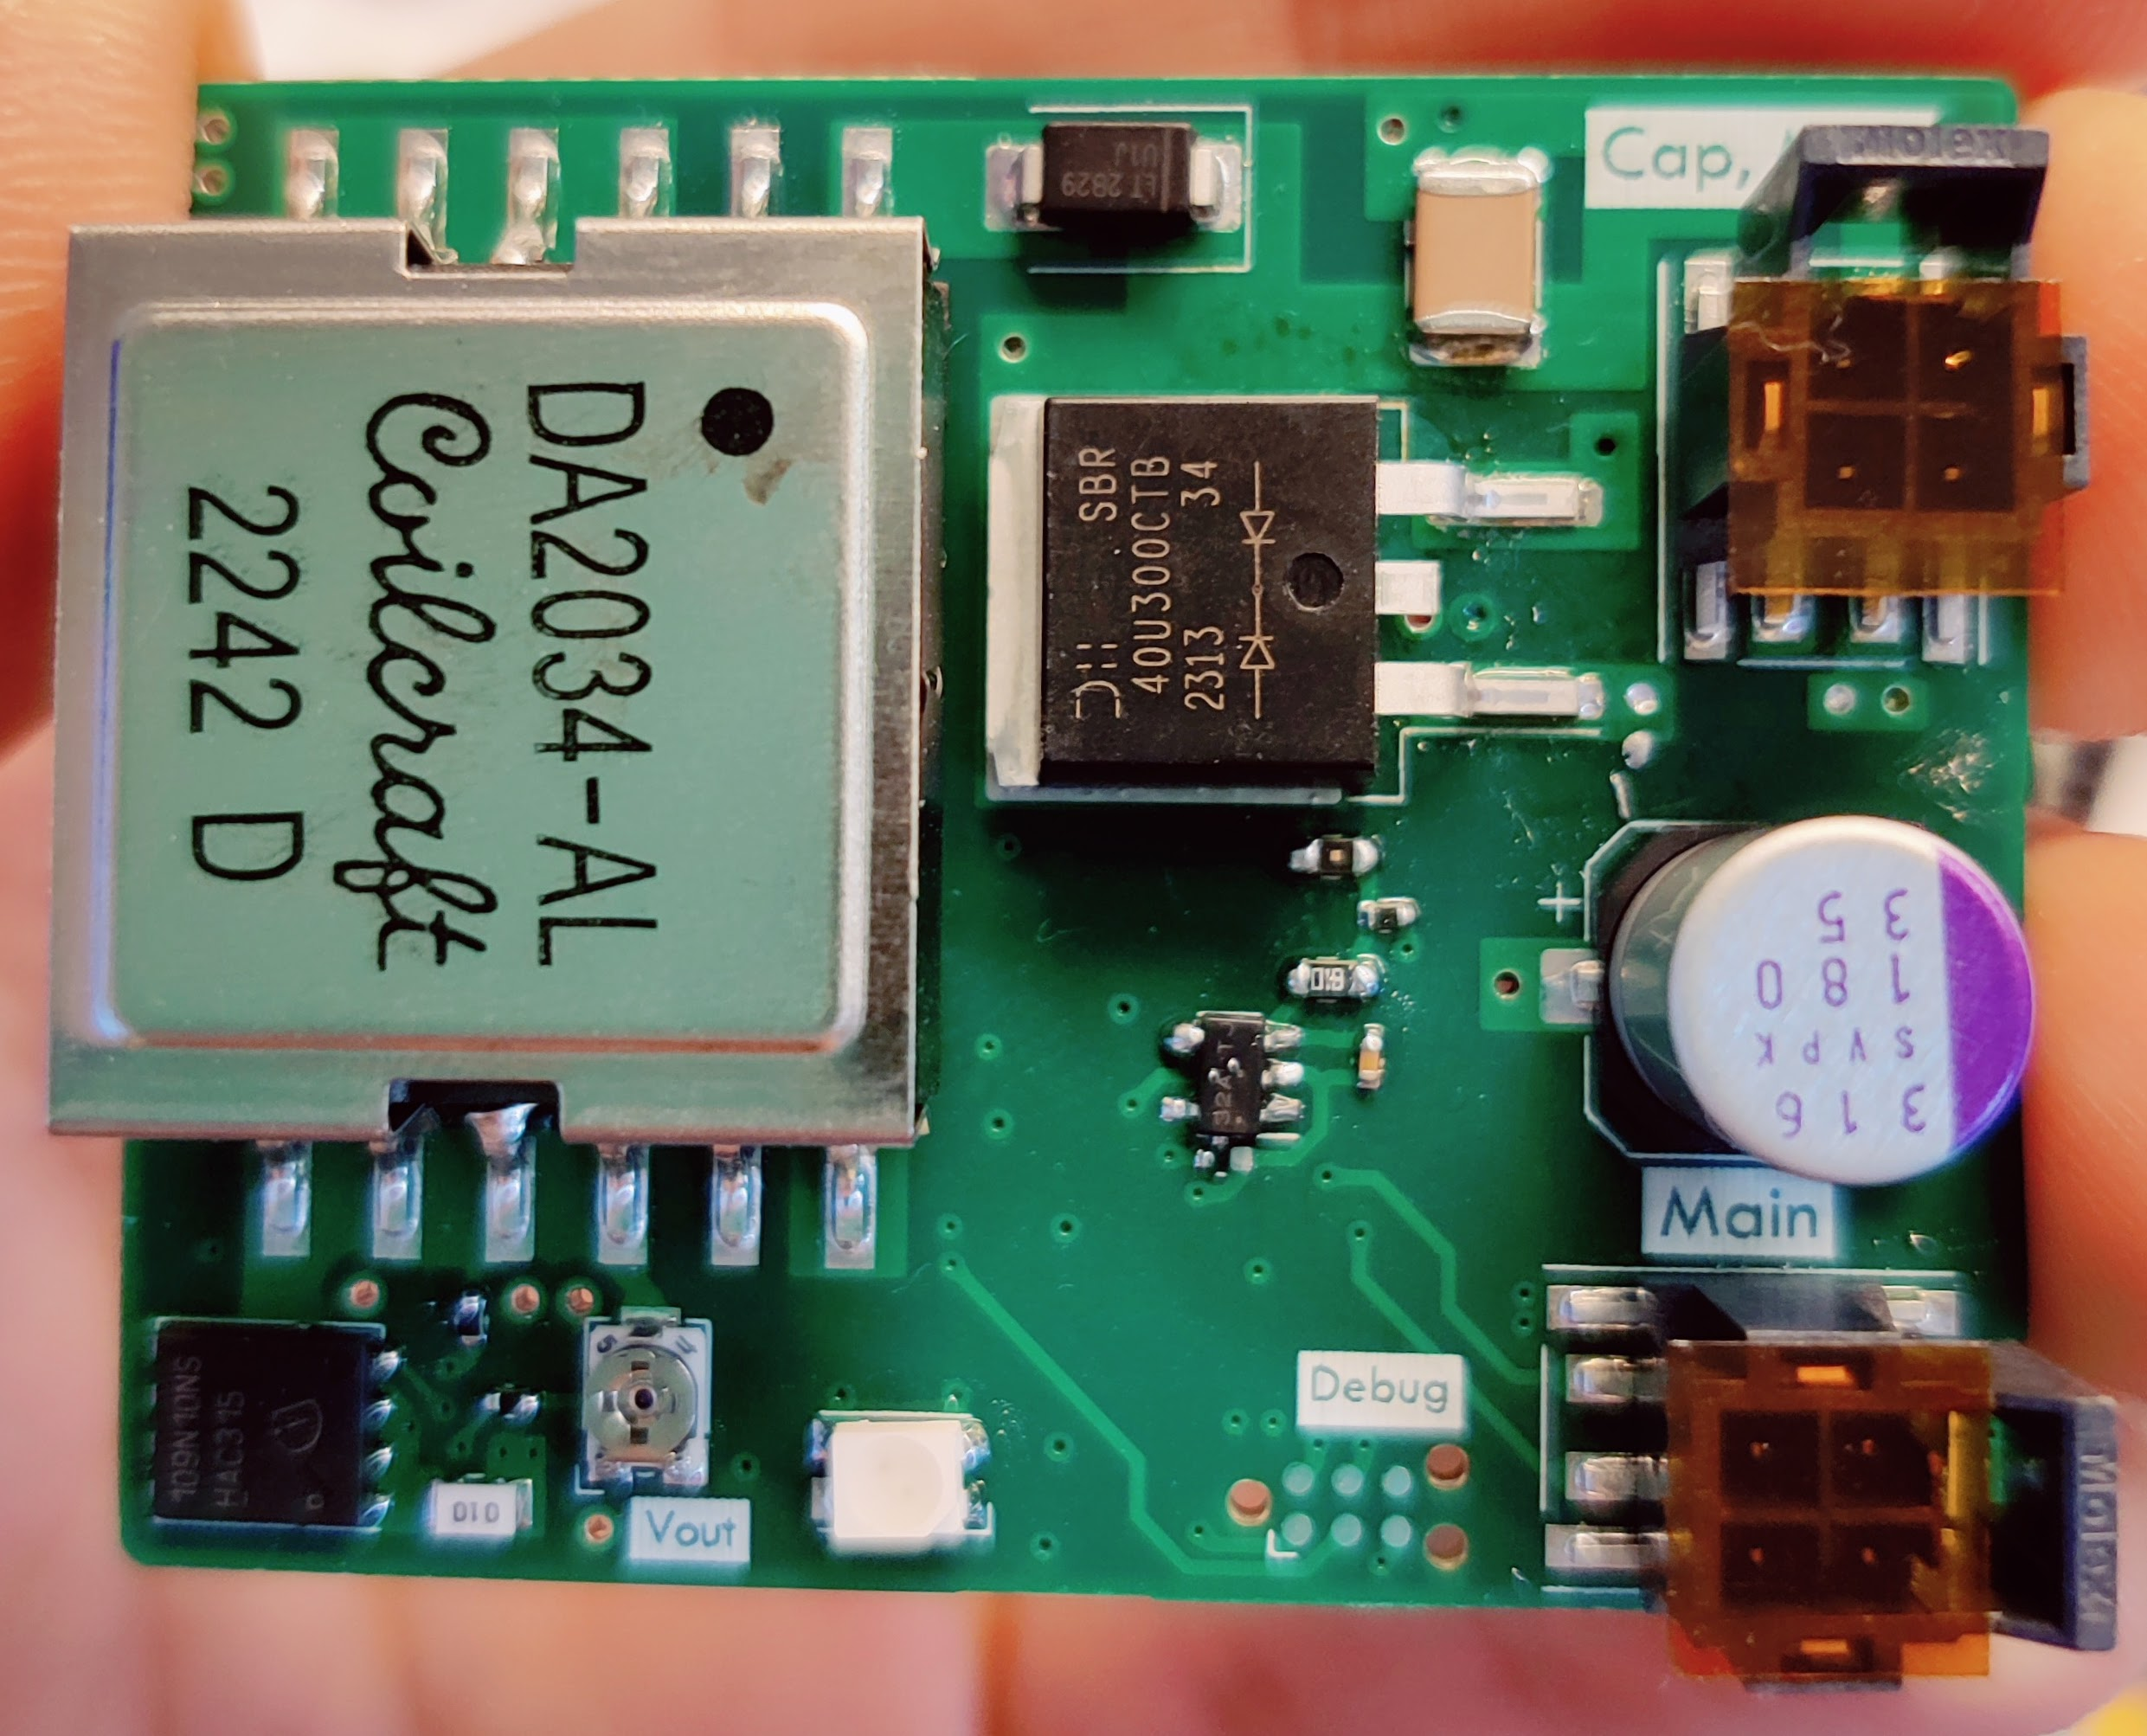
\includegraphics[width=0.8\textwidth]{images/mikona.jpg}
    \caption{The new kicking board design}
    \label{fig:mikona}
\end{figure}

After writing our last year's TDP, we switched to a simpler PIC microcontroller instead of the STM32. This resulted in major simplification that improved both reliablity and the cost.

We also have a high-power resistor network. It consists of three 2.4K 3W resistors. It discharges the capacitors when needed, without using the kicker magnets. The STN3N40K3 MOSFET driven by a ZXGD3009E6 is used to control the discharge.

For the actual kicking, two IGB50N60T IGBTs driven by a single IX4427MTR are used to discharge the capacitors to the kicking magnets.

It is also worth mentioning that the variable programmable resistor was removed after writing last year's TDP. This was because it was not necessary. The boost voltage rarely changes. When it does change, it usually involves a corresponding hardware change. At that time, we can simply re-calibrate the mechanical variable resistor instead.

\section{Software}
Last year we started to rewrite our software (Fig. \ref{fig:software-architecture}), focusing on the following points:

\begin{figure}
    \centering
    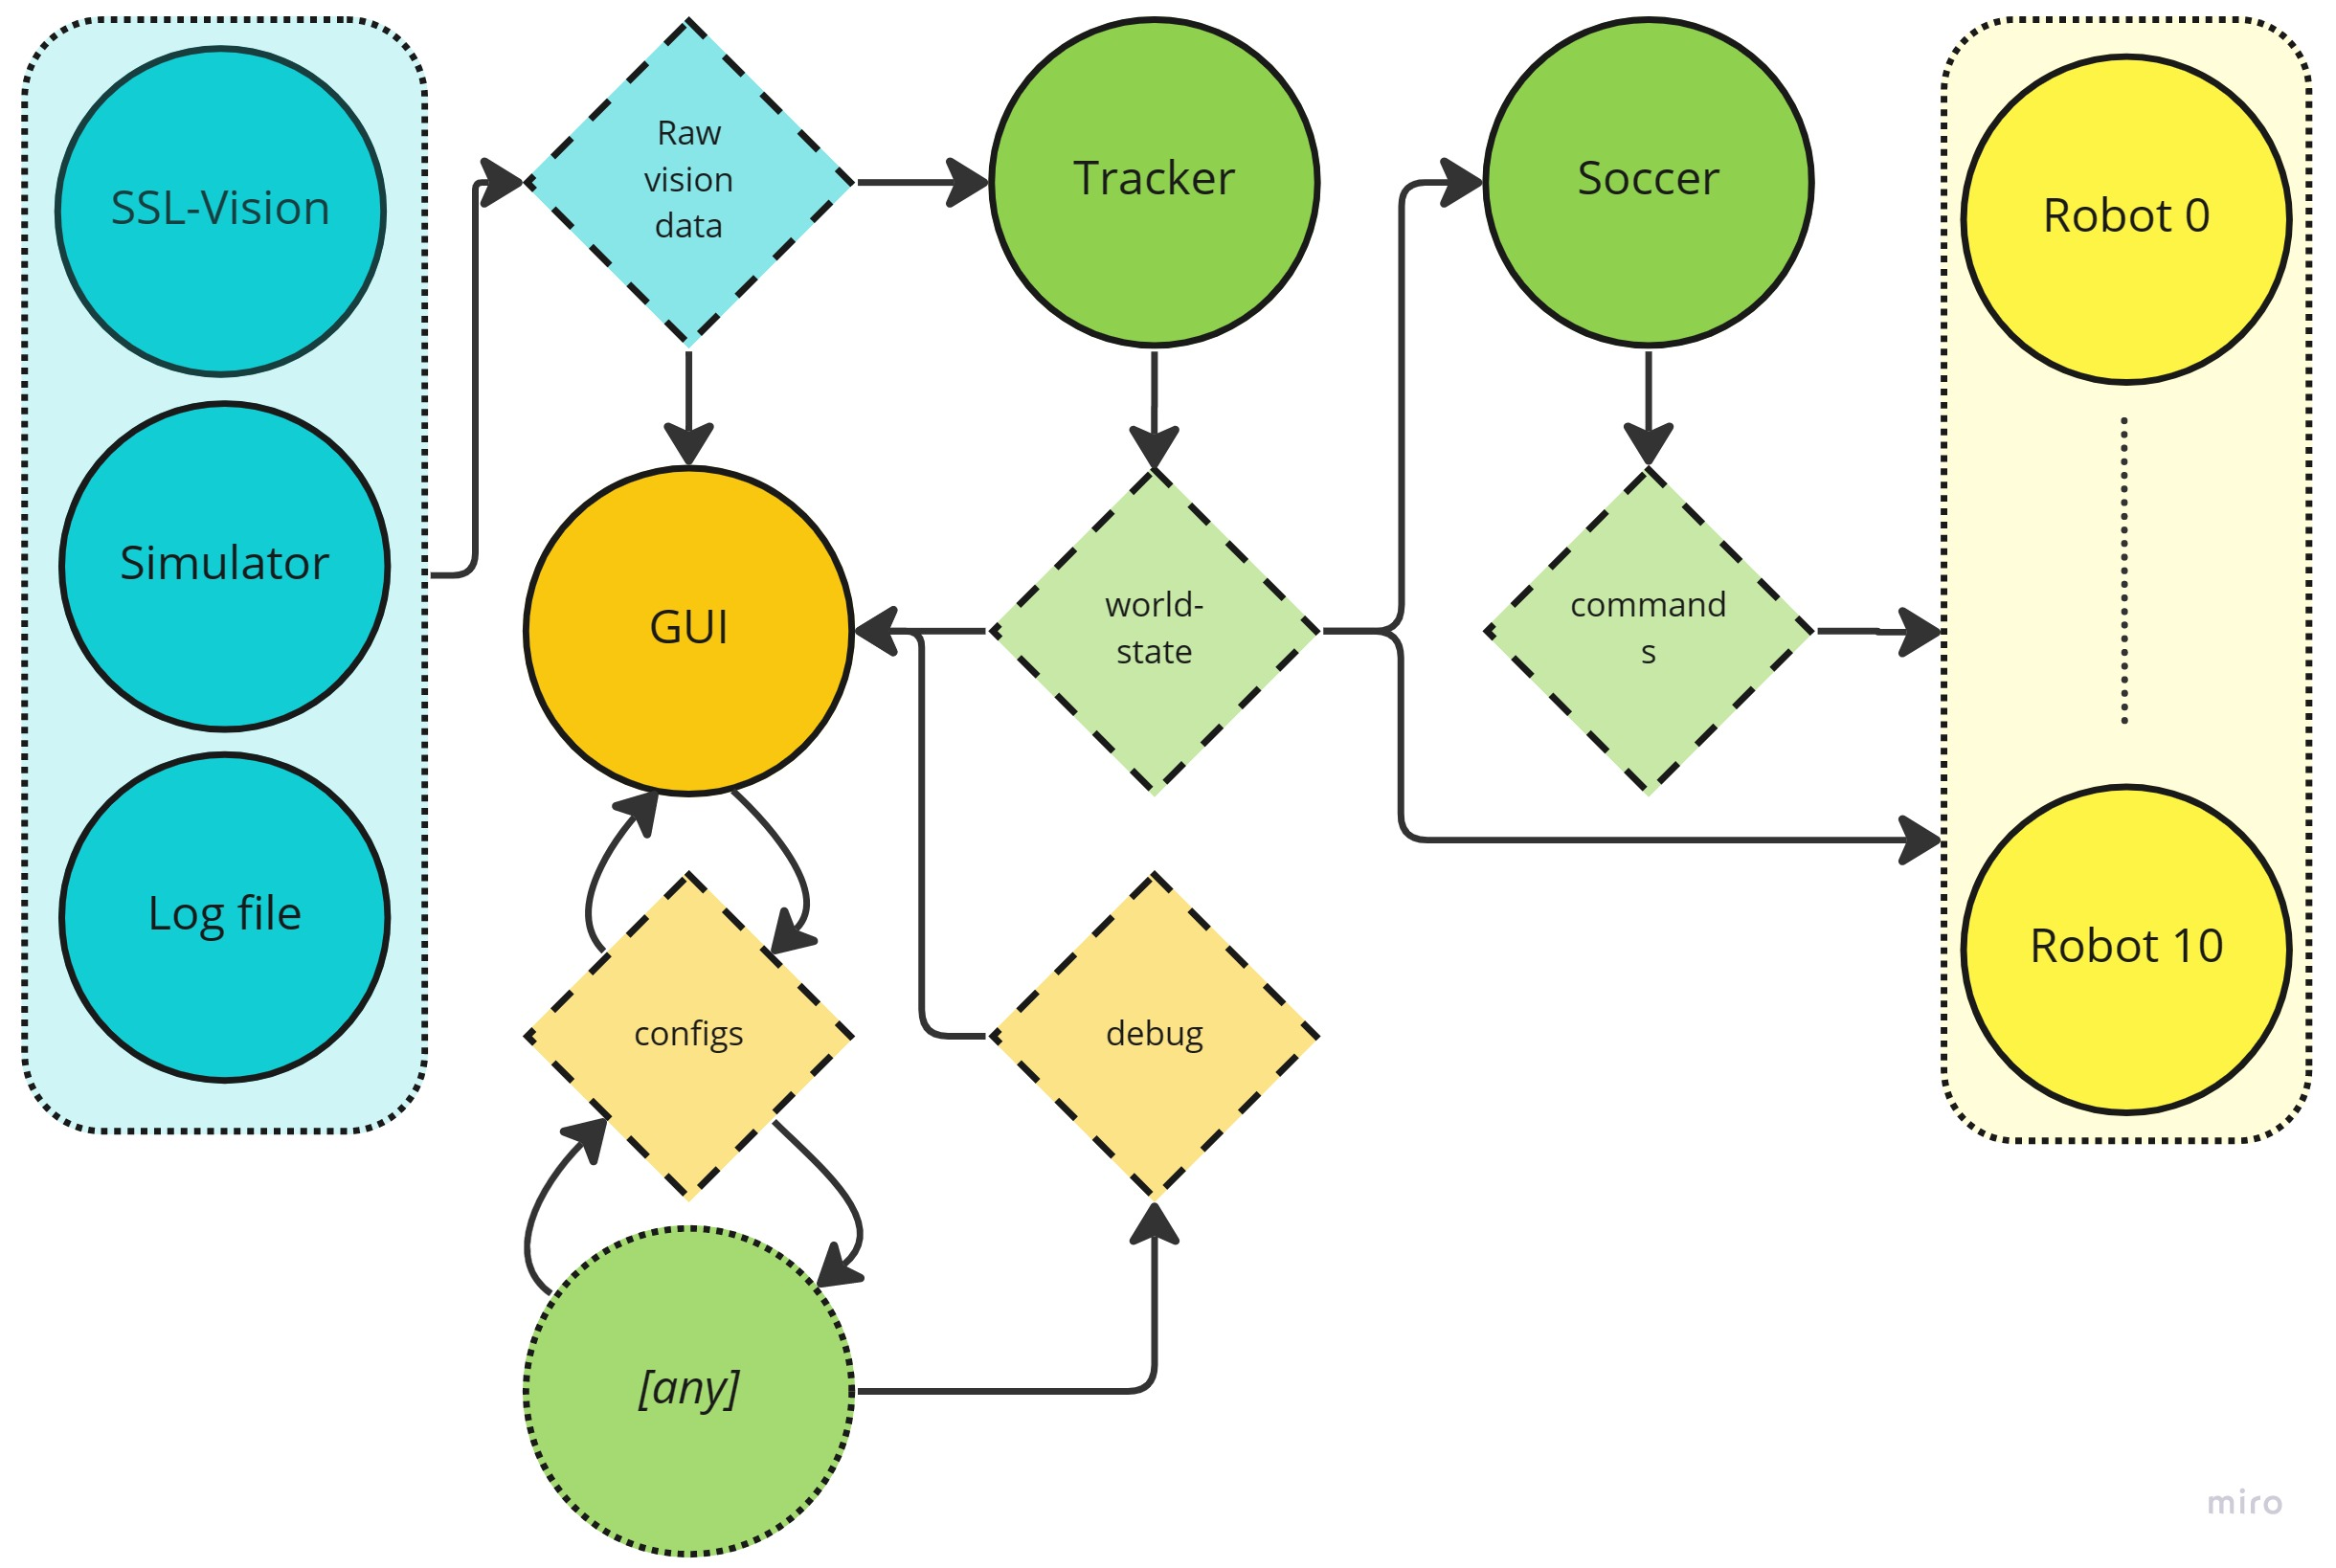
\includegraphics[width=0.8\textwidth]{images/software-architecture.jpg}
    \caption{The new software architecture}
    \label{fig:software-architecture}
\end{figure}

\begin{enumerate}
    \item more robust
    \item easier to read and understand
    \item faster to iterate and extend
    \item more competitive
\end{enumerate}

We managed to finish the rewrite and successfully test it in the simulator. However, using the new software during the real competition surfaced a huge number of issues. In the end we reverted to the old software, while cherry-picking parts of the development from the new rewrite.

In the following sections, we will describe the issues we faced, and ways we are planning to tackle them.

\subsection{Motion control}
Developing effective robot motion control systems presents a multifaceted challenge. This is especially true when relying only on simulated environments as test-beds. Our initial attempt at this endeavor encountered significant hurdles. These were primarily due to the inherent limitations of simulators. Simulators struggle to capture the complexities of real-world dynamics. They often fail to accurately represent the intricate interplay of physical forces. Also, they struggle with sensor noise and environmental uncertainties. These factors influence robot behavior. Controllers designed and optimized in simulation frequently falter when deployed on physical robots. This leads to suboptimal performance or outright failure.

In our previous endeavor, we faced the repercussions of this disparity firsthand. Despite promising results in simulation, our motion control algorithms proved ineffective when transferred to real robots, highlighting the inadequacy of our approach. However, rather than viewing this setback as a failure, we recognized it as an invaluable learning opportunity. Leveraging the data collected from our physical robots during last RoboCup, we gained valuable insights into the nuanced challenges and discrepancies between simulation and reality. This dataset, comprising observations of real-world interactions, sensor readings, and system responses, serves as a rich repository of information for refining our motion control strategies.

Building upon this foundation, our current approach integrates the lessons learned from our past shortcomings. We aim to develop motion control algorithms that are not only robust in simulation but also resilient in real-world scenarios. By incorporating the empirical knowledge gleaned from physical robot experiments, we seek to ensure that our controllers exhibit consistent performance across both domains. Through a data-driven methodology, we strive to create motion control systems that are adaptable, responsive, and capable of navigating the complexities of dynamic environments with precision and reliability.

\subsection{Alternative Programming Languages}
In our pursuit of refining our software, we recognize the pivotal role that programming languages play in facilitating efficient development workflows and minimizing error-prone coding practices. While C++ has traditionally served as a cornerstone language for robotics due to its performance and versatility, its stringent memory management requirements and relatively slow iteration times present significant drawbacks. Therefore, we are actively exploring alternative programming languages that offer enhanced development iteration and are more accessible to beginner programmers, while also mitigating the pitfalls associated with manual memory management.

A key criterion in selecting a new programming language is its ability to support hot-reloading, thereby enabling rapid iteration and experimentation without the need for time-consuming recompilation cycles. Hot-reloadable languages empower developers to make real-time changes to code and see immediate results, fostering a highly iterative development process that accelerates prototyping and debugging. This capability is particularly valuable in the context of refining robot motion control, skills, and plays, where quick iteration is essential for fine-tuning algorithms and adapting to evolving requirements.

Moreover, prioritizing ease of use is paramount, as it lowers the barrier to entry for novice programmers and streamlines the learning curve associated with robotics development. By selecting a language with intuitive syntax and comprehensive documentation, we aim to foster a more inclusive and accessible development environment, where individuals from diverse backgrounds can contribute effectively to our projects.

Furthermore, we seek a language that offers robust memory management mechanisms to mitigate the risk of common pitfalls such as memory leaks and segmentation faults, which are prevalent in C++ due to its manual memory allocation and deallocation model. A less error-prone language in this regard would not only enhance code reliability but also reduce development overhead associated with debugging memory-related issues.

Currently, we are actively experimenting with several candidate languages, including \textbf{\textit{Lua}} \cite{ref_3rd-lua}, \textbf{\textit{V}} \cite{ref_3rd-v-lang}, and \textbf{\textit{Odin}} \cite{ref_3rd-odin}, each of which offers unique features and advantages that align with our development objectives.

\newpage
\begin{thebibliography}{8}

\bibitem{ref_ETDP2023}
Immortals 2023 Extended Team Description Paper, \url{http://tinyurl.com/4xt23jb8}.

\bibitem{ref_github}
Immortals Open Source Project. \url{https://github.com/Immortals-Robotics}.

% 3rd-party libraries
\bibitem{ref_3rd-lua}
Lua, embeddable scripting language \url{https://www.lua.org/}

\bibitem{ref_3rd-v-lang}
The V Programming Language \url{https://vlang.io/}

\bibitem{ref_3rd-odin}
Odin Programming Language \url{https://odin-lang.org/}

\end{thebibliography}
\end{document}
